% Исходный LaTeX-код (c) Пётр Калинин
% Код распространяется по лицензии GNU GPL (!)

\lheader{Кодировки и работа с ними}

\epigraph{This coded character set is to facilitate
the general interchange of information
among information processing systems,
communication systems, and
associated equipment.\\
\dots An 8-bit set was considered
but the need for more than 128 codes
in general applications was not yet evident.
\footnote{\textit{Этот набор символьных кодов должен облегчать общий обмен информацией 
между вычислительными системами, системами связи и соответствующим 
оборудованием
\dots Был рассмотрен 8"=битный набор, но необходимость иметь более 128 кодов в 
общих приложениях пока ещё не очевидна.}\\
Цитата (и русская, и английская) взята из \TeX book}
}
{ASA SUBCOMMITTEE X3.2,\\
American Standard Code for Information Interchange (1963)\\
}

Как вы прекрасно знаете, любые данные, с которыми работает компьютер, "--- это 
просто последовательность \textit{байт}, т.""е. чисел, каждое от 0 до 255. 
Трактовка того, что каждое из этих чисел обозначает, целиком зависит от 
приложения.

Но нередко возникает необходимость работать с \textit{текстом}, который нужно так или 
иначе показывать пользователю. Для этого необходимо уметь как"=то 
последовательность чисел перевести в последовательность картинок, которые 
человеком будут опознаны как буквы. Конкретный внешний вид каждой картинки 
определяется, конечно, \textit{шрифтом}, но все"=таки необходимо иметь 
некоторую договорённость о том, как последовательность чисел переводится в 
буквы (хотя бы чтобы во всех шрифтах буква A была в одном и том же месте).      
Эта договорённость, вообще говоря, и называется \textit{кодировкой}, или \textit{кодовой таблицей},
или \textit{кодовой страницей} (codepage), и про 
различные кодировки я и буду говорить в этом параграфе.

\note{Конечно, наличие такой фактически устной договорённости ничего ровным 
счётом не обозначает. Вполне может найтись шрифт, в котором соответствие между 
числами и буквами не то "--- и с этим шрифтом все будет плохо. Более того, в 
принципе, можно вручную "<подломать"> тот или иной шрифт "--- и вы увидите, как 
все испортится.}

Ещё одно замечание: я рассказываю тут все так, как я это понимаю. Конечно, 
я не претендую на абсолютную точность, особенно в исторической части.

По"=видимому, одним из первых таких "<соглашений">, стандартов был American Standart 
Code for Information Interchange, ASCII. Он определял размер байта равным 7 битам и, соответственно, определял значения 128 символов. Эти 128 символов и 
до сих пор неизменны и в любой кодировке (по крайней мере из тех, с которыми вы 
в первую очередь столкнётесь :) ) следуют таблице ASCII. Первые 32 из них
имели (и в основном до сих пор имеют) особое, внутри"=компьютерное значение и 
потому являлись (и до сих пор считаются) так называемыми \textit{управляющими}, 
или \textit{служебными} символами; о них я скажу чуть ниже.  Остальные же 
числа соответствуют различным частоупотребляемым символам, цифрам и латинским 
буквам. Это соответствие (какому числу, т.е. какому коду, соответствует какая 
буква) вы легко можете увидеть: как просто написав простую программу на 
паскале: chr(i) "--- это символ с номером i, "--- так и посмотрев в "<Таблице 
символов"> "--- стандартной программе Windows (Пуск "--- Стандартные "--- 
Служебные "--- Таблица символов), но там управляющие символы не рисуются; а ещё 
есть плагин к Far'у "--- Character Map, можете поставить и посмотреть.
    
Немного ещё скажу про управляющие, или служебные, символы. Изначально кодировка, 
видимо, предназначалась непосредственно для передачи данных между разными устройствами; например, видимо, вывод данных на принтер 
осуществлялся просто копированием текста в порт принтера. При этом все неуправляющие коды 
напрямую переводились в картинки и выводились на экран или на печать, а управляющие символы 
не выводились, а именно управляли процессом вывода (т.е. драйвер монитора/принтера 
трактовал эти символы особым образом). Конечно, каждому символу также 
соответствует некоторая картинка (например, рожицы),  
но также и некоторое действие. Теперь эти действия работают в основном только при выводе текста в 
консольное окно, но все равно они имеют смысл. Можете с ними поэкспериментировать. Перечислю смысл некоторых символов:
\begin{ulist}                                                                 
\item Символ \#7: Beep: не выводит ничего на экран, но издаёт звуковой сигнал (писк) системным динамиком.
Очень удобное средство издавания звука, например: \texttt{writeln(\#7'An error occcured!');}
\item Символ \#8: а-ля backspace: передвигает курсор на позицию влево (но не стирает символ, который был 
в той позиции!) Например, \texttt{write('a'\#8);} выводит символ \texttt a и оставляет курсор \textit{под}
этим символом, а потому \texttt{write('a'\#8'b');}\footnote{Обратите внимание, как вставлять символы, заданные кодами, в строки в паскале} в итоге эквивалентно \texttt{write('b');}
\item Символ \#9: Tab: передвигает курсов вправо до ближайшей позиции, кратной восьми (при выводе на экран,
насколько я понимаю; другие программу при желании могут до вывода на экран заменять этот символ на нужное им 
число пробелов). Вообще, это один из немногих управляющих символов, который, насколько я понимаю, активно
используются и сейчас везде, позволяя приложениям выравнивать текст как они хотят.
\item Символ \#10: Line feed: перемещает курсор на строку вниз, \textit{оставляя его в том же столбце}.
\item Символ \#13: Carriage return: возвращает курсор в начало текущей строки.
\item Символ \#26: EOF (end of file): конец файла. Видимо, подразумевалось, что это будет последний символ в файлах
(хотя я далеко не уверен). На самом деле он сейчас в основном, видимо, используется как символ окончания ввода, 
да и то редко.
\end{ulist}

Символы с номерами от 1 до 26 также иногда называют соответственно Ctrl-A, Ctrl-B, \dots, Ctrl-Z (т.е.,
в частности, Ctrl-Z "--- это EOF, потому ввод с клавиатуры в команде \texttt{copy con file} надо заканчивать именно
символом Ctrl-Z).  Это скорее просто обозначение (т.е. это не значит, что всегда по нажатию на клавиатуре Ctrl-Z будет введён 
символ EOF, а по Ctrl-A "--- символ \#1 "--- для этого нужна особая обработка программой), причём это обозначение используется весьма редко, но его все
равно полезно помнить.

Ещё особые слова про символы номер 10 и 13. Видимо, первые принтеры были устроены как печатающие машинки, и, чтобы 
начать печать новой строчки, надо было сделать две операции: прокрутить лист бумаги на строчку вниз ("<скормить">
принтеру одну строку бумаги :) "--- line feed), при этом столбец, где находился курсор, не изменится "--- и 
передвинуть печатающую каретку в начало строки "--- carriage return. Потому для перевода строки использовались именно 
два символа "--- 13 (CR) и 10 (LF). С тех пор многое изменилось. Теперь символы имеют скорее условный смысл, и в Windows
просто "<по договорённости"> принят перевод строки как последовательность из двух символов "--- 13 и 10. В Unix"=системах используется перевод 
только одним символом (13, если не ошибаюсь). В этом смысле говорят от форматах файлов Windows и UNIX "--- различие только
в том, как обозначается перевод строки. Но по"=прежнему в Windows при выводе 
\textit{в консольное окно} (т.""е. в текстовое окно) символы 13 и 10 имеют 
различные значения: именно то, что написано выше. Если с начала строки вывести 
\texttt{write('abc'\#13'd');} то получится \texttt{dbc} и курсор будут под \texttt{b}.

Позже стало ясно, что 7 бит не хватает для обозначения всех нужных символов, и стали использовать 8 бит на байт, что позволило иметь ещё 128 символов.
Видимо, довольно быстро придумали, 
что там нужно иметь: туда поместили западноевропейские символы (типа \` a, \c c и т.п.), а также символы псевдографики
(которыми рамочки рисуются) и т.п. Получилась западноевропейская кодировка. (Я точно не знаю, существуют ли различные варианты 
западноевропейской кодировки, поэтому много про неё писать не буду).

Когда в России (СССР ещё, видимо) решили придумать кодовую таблицу, конечно, за основу решили взять таблицу ASCII и просто
поместить русские буквы во второй половине таблицы. Я не буду, наверное, давать тут подробный обзор, только перечислю 
три наиболее распространённые русские кодировки:

\begin{ulist}                         
\item Кодировка DOS, или cp866 (вообще, насколько я понимаю, Microsoft или кто-то ещё занумеровали почти все существующие
кодировки "--- не только русские, но и другие). Эта кодировка была придумана, видимо, ещё в СССР и широко использовалась в 
DOS и до сих пор используется в консольном выводе в Windows. Взяли западноевропейскую кодировку и заменили в ней 
западноевропейские символы на русские, сохранив псевдографику на местах. Правда, при таком условии не нашлось два блока
по 32 свободных символа подряд, поэтому все русские заглавные буквы тут идут подряд в алфавитном порядке, а вот маленькие
разбиты на две группы по 16 символов: а--п и р--я вроде. В каждой группе символы идут подряд в алфавитном порядке,
но между п и р идут около 32 символов псевдографики.
\item Кодировка KOI8-R. Тоже изобретена давно. Основное её свойство "--- если у кода русской буквы отбросить старший бит,
то получится (в большинстве случаев) некая похожая английская буква. Т.е. раз символ номер 61 "--- латинская А, то символ номер 
128+61 "--- русская А; 62 "--- английская B, тогда 128+62 "--- Б и т.д. В результате русские буквы идут в неалфавитном порядке,
но зато если некое устройство умеет выводить только первые 128 символов, то отбросив первый бит, получим хотя
бы читабельный текст (типа Russkij Tekst). Используется сейчас в первую очередь иногда в 
e-mail и почему-то в Linux и т.п. (Существует ещё и KOI8-U "--- украинская, насколько я понимаю.)
\item Кодировка Windows, она же cp1251 или прямо Windows"=1251. Её, видимо, придумало Microsoft для использования
в Windows. Здесь и маленькие, и заглавные русские буквы идут сплошными блоками, без разрывов в 
алфавитном порядке. Используется довольно часто в Windows (хотя нередко вытесняется Unicode, 
см. ниже).
\end{ulist}

Естественно, общих символов, т.е. символов, которые присутствуют во всех трёх кодировках (точнее, во 
вторых половинах всех трёх кодовых таблиц), не 
так уж и много: это, конечно же, все русские буквы (за исключением, возможно, буквы Ё, 
которая, может быть, не присутствует в KOI8-R), а также, может быть, ещё несколько символов 
типа `№', поэтому не имеет смысла говорить о взаимно"=однозначном соответствии между 
кодировками. Но, с другой стороны, в текстах из всей второй половины таблицы в основном используются 
только русские буквы, и в этом смысле можно говорить о \textit{перекодировке} текста из одной 
кодировки в другую: т.е. о замене в тексте одних чисел (значений байтов) на другие, которые 
соответствуют той же букве, но в другой кодировке. Ещё раз подчеркну, что перекодировка корректно 
переведёт только русские буквы и, может быть, ещё некоторые символы, но с остальными символами
(например, псевдографика из кодировки DOS) ничего толкового сделать не получится: аналогичный 
символ просто будет отсутствовать в целевой  кодировке (что произойдёт в этом случае, зависит, конечно, 
от самой программы перекодировки; например, она может заменить все такие символы на знаки 
вопроса и т.п.).

Уточню, что обозначает слово "<используется"> в тексте выше. На самом деле оно обозначает именно то,
что обозначает: что в этих случаях русские буквы кодируются именно в соответствии с данной
кодировкой. Например, я несколько раз получал e-mail, в которых, если поглядеть в их исходный текст,
русский текст был написан в кодировке KOI8-R. Конечно, прежде чем выводить текст на экран,
программа работы с электронной почтой перекодировывала текст. Фраза "<используется при выводе в
консоль"> обозначает, что, если вы будете выводить текст в консольное окно (т.е. текстовое окно), то
текст будет преобразовываться в картинки в соответствии с этой кодировкой (т.е. будет 
использоваться соответствующий шрифт). И т.п.

\begin{center}
\hrule

\vspace{0.2cm}
{\footnotesize 
      
\begin{tabular}{ccc}
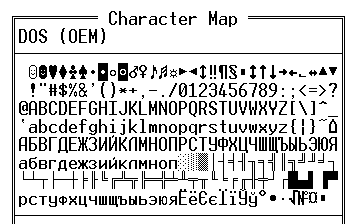
\includegraphics[width=5cm,height=3.128cm]{ideas/03_1_encodings/dos.png}&
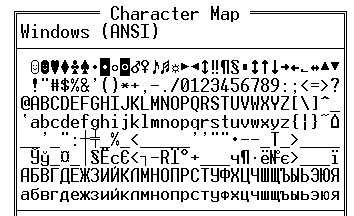
\includegraphics[width=5cm,height=3.128cm]{ideas/03_1_encodings/win.png}&
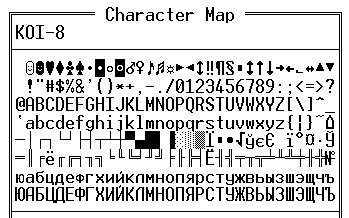
\includegraphics[width=5cm,height=3.128cm]{ideas/03_1_encodings/koi.png}\\
DOS (cp866)&Windows-1251&KOI8-R
\end{tabular}

Кодировки (первая строка "--- символы номер 0.\,.31, вторая "--- 32.\,.63 и т.д.). Получено просто 
с плагина Character Map к Far. Во второй половине таблицы в DOS корректно показаны все символы, в 
остальных таблицах "--- в основном только русские буквы, остальные символы могут быть неправильные. 
Зацените порядок русских букв в KOI8-R.

}

\vspace{0.2cm}

\hrule
\end{center}

Но со временем стало ясно, что 8 бит для представления текстов мало. Поэтому была изобретена 
\textit{кодировка Unicode}. В отличие от всех остальных распространённых сейчас кодировок, она не подразумевает 
использования 8 бит на символ.  Наиболее распространены, видимо, три варианта кодировки Unicode: 
\begin{ulist}
\item UTF-8, в которой на наиболее часто используемые символы (а именно, первую половину таблицы ASCII) 
используется один байт (8 бит, первый из которых 0), на некоторые символы (в т.ч. русские) "--- два байта (при этом, 
естественно, так, чтобы нельзя было перепутать с однобайтовыми символами "--- первый бит первого 
байта обязательно 1), а на некоторые "--- три или четыре (всегда по первым битам первого байта можно 
различить, какой из этих четырёх случаев имеет место). 
\item UTF-16: в ней часть символов занимает 2 байта, а часть "--- четыре. Я ни разу не помню, чтобы 
встречал эти четырехбайтовые символы, поэтому в первом приближении можно пренебречь их 
существованием и считать, что каждый символ UTF-16 занимает два байта.
\item UTF-32: все символы кодируются 4 байтами. Я лично сталкивался с этой кодировкой очень редко.
\end{ulist}
Кодировки Unicode сейчас весьма распространены (и вообще, есть люди, которые считают, что использовать
где-либо что-либо кроме Unicode нельзя, но я с ними до конца не соглашусь). Ещё замечу, что во всех 
этих кодировках возникает так называемая проблема 
byte endianness "--- проблема порядка байт: если на символ требуется больше одного байта, то какой 
из них писать первым, а какой вторым. Иногда пишут одним способом, иногда другим (на самом деле это 
проблема не только кодировки, но и вообще представления чисел).\footnote{\textit{Термины big-endian и little-endian первоначально не имели отношения к информатике. 
В сатирическом произведении Джонатана Свифта "<Путешествия Гулливера"> описываются вымышленные 
государства Лилипутия и Блефуску, в течение многих лет ведущие между собой войны из-за разногласия 
по поводу того, с какого конца следует разбивать варёные яйца. Тех, кто считает, что их нужно 
разбивать с тупого конца, в произведении называют "<Big-endians"> ("<тупоконечники">).} "--- 
\texttt{http://ru.wikipedia.org/wiki/Порядок\_байтов}}

И финальные замечания: если вы видите, что какой-то текст, который, как вы думали, должен быть 
нормальным русским текстом, выглядит набором странных символов, то, скорее всего, вы смотрите его в 
неправильной кодировке. Как правило, правильная кодировка "--- это одна из перечисленных выше. Если 
вы столкнулись с этой проблемой, просматривая сайт или электронную почту, то, как правило, это не 
составляет проблемы: большинство браузеров и почтовых программ позволяют вручную указать кодировку, 
в которой следует просматривать текст (т.е. они перед выводом на экран перекодируют текст из 
указанной кодировки). Если же это текстовый файл, то: Far 1.x благополучно умеет показывать кодировки 
Windows, DOS, а, если его подучить, то и KOI8-R (смотрите каталог \verb|Far\Addons\Tables\Cyrillic| при
желании). Unicode он может только показывать UTF-16, поэтому, что делать с Unicode, если его надо 
вручную редактировать или просматривать UTF-8 или UTF-32, однозначно посоветовать не могу. Можно 
открыть файл в браузере и вручную попросить нужную кодировку.

Наконец, приведу результаты просмотра текста `\texttt{Russian text Русский текст}', написанного 
изначально в разных кодировках, в кодировке DOS (т.е. изначальный текст я написал в разных 
кодировках, а потом стал просматривать в DOS):

\begin{center}
\hrule

\vspace{0.2cm}
\noindent\begin{tabular}{c|c|c}

\includegraphics[width=5cm,height=0.4cm]{ideas/03_1_encodings/rustext_dos.png}&
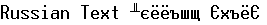
\includegraphics[width=5cm,height=0.4cm]{ideas/03_1_encodings/rustext_win.png}&

\includegraphics[width=5cm,height=0.4cm]{ideas/03_1_encodings/rustext_koi.png}\\
DOS&Windows&KOI8-R
\end{tabular}

\vspace{0.2cm}
\hrule
\vspace{0.2cm}

\noindent\begin{tabular}{c|c}
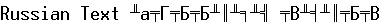
\includegraphics[width=7cm,height=0.4cm]{ideas/03_1_encodings/rustext_utf8.png}&

\includegraphics[width=9cm,height=0.4cm]{ideas/03_1_encodings/rustext_utf16.png}\\
UTF-8&UTF-16
\end{tabular}
\vspace{0.2cm}
\hrule
\end{center}

(Разные пропорции у разных символов "--- это ничего не значит, мне просто лень было подбривать 
размеры при вставке картинок в текст.) Конечно, текст, изначально написанные в кодировке DOS, 
нормально вполне в этой кодировке и просматривается; особых комментариев по тексту, изначально 
написанному в кодировках Windows и KOI8-R, я не придумал, но обратите внимание на следующие 
особенности Unicode-кодировок:


\begin{ulist}
\item UTF-8.  Обратите внимание, что английский текст (и все три пробела!) получился вполне нормальным, и только русский 
текст испортился. Обратите также внимание на некоторую довольно заметную двухбайтную периодичность 
в русском тексте
(т.е. на то, что чётные байты довольно сильно отличаются от нечётных: в чётных байтах встречаются 
то буквы, то символы псевдографики, а в нечётных "--- только два разных символа псевдографики).
Это общий признак кодировки UTF-8: если вы видите, что все английские буквы, 
цифры, знаки препинания и т.п. выглядят нормально, а вот там, где должны быть русские буквы, 
написана какая-то чушь с явной двухбайтовой периодичностью, то скорее всего, вы просматриваете 
кодировку UTF-8. Для примера картинка: отрывок из xml-файла, записанного в кодировке UTF-8 и 
просмотренного, на этот раз, в кодировке Windows. Все, кроме русских букв, как будто в однобайтовой 
кодировке, а в русских буквах явно видна периодичность в два байта. Обилие подчерков объясняется 
тем, что этим кодам в Windows-кодировке соответствуют одинаковые изображения (т.е. что в 
Windows-кодировке на этом месте не находятся никакие толковые символы типа русских букв и потому
этим символам не стали придумывать никаких умных картинок; та же причина, что и в обилии подчерков в
приведённой выше таблице символов для кодировки Windows).
\begin{center}
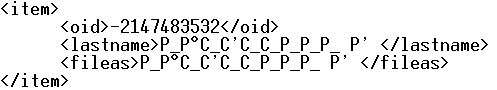
\includegraphics[width=8cm,height=1.44cm]{ideas/03_1_encodings/utf8_contact.png}
\end{center}

\item UTF-16. Обратите внимание, что на этот раз \textit{все} символы занимают по два байта. И 
английские, и русские буквы, и пробелы занимают два байта; при этом первый байт у английских букв и 
пробелов "--- символ номер ноль (который в этом шрифте имеет такую же картинку, что и пробел, и 
потому выглядит как пробел), а второй байт как раз и есть соответствующий символ (английская буква 
либо символ 32 для пробела). Первый байт у русских букв, как вы можете видеть из таблиц кодировок 
выше, есть символ номер 4, ромбик. Этот ромбик на самом деле является характерным признаком 
русского текста, написанного в кодировке UTF-16 и просматриваемого в однобайтовой кодировке (что 
DOS, что Windows), а "<разрежённые"> английские буквы и цифры (на самом деле, ещё раз, между ними 
не пробелы, а символы номер 0) "--- характерным признаком английского текста в кодировке Unicode. 
Ещё раз подчёркиваю, что, т.""к. вы, скорее всего, не будете сталкиваться с четырехбайтовыми 
символами в UTF-16, то можно приближённо считать, что UTF-16 "--- абсолютно двухбайтовая кодировка.
\end{ulist}

\note{Почему я привожу все отрывки здесь в виде картинок. Потому что в \TeX{}е используется на 
самом деле своя кодировка; при чтении входного файла он осуществляет перекодировку из входной 
кодировки в свою, при этом часть символов, естественно, теряется. Поэтому, чтобы донести до вас по 
возможности полное многообразие символов разных кодировок, я их вставляю картинками.}